\PassOptionsToPackage{unicode}{hyperref}
\documentclass[aspectratio=1610, professionalfonts, 9pt]{beamer}

\usefonttheme[onlymath]{serif}
\usetheme[showtotalframes]{tudo}


\usepackage{polyglossia}
\setmainlanguage{english}

% Mathematik
\usepackage{mathtools}

% Enable Unicode-Math and follow the ISO-Standards for typesetting math
\usepackage[
  math-style=ISO,
  bold-style=ISO,
  sans-style=italic,
  nabla=upright,
  partial=upright,
]{unicode-math}
\setmathfont{Latin Modern Math}

% nice, small fracs for the text with \sfrac{}{}
\usepackage{xfrac}

\usepackage{multicol}
\usepackage{graphicx}
\usepackage{amssymb}
\usepackage{amsmath}
\usepackage{xparse}
\usepackage{braket}
\usepackage{units}
\usepackage[locale=DE,separate-uncertainty=true,per-mode=reciprocal,output-decimal-marker={,},]{siunitx}
\sisetup{
  round-mode          = places, % Rounds numbers
  round-precision     = 2, % to 2 places
}
\usepackage[section]{placeins}
\usepackage{pdflscape}
\usepackage{expl3}
\usepackage{bookmark}
\usepackage{booktabs}
%Komma als Dezimaltrenner in der mathe Umgebung, um in Umgebungen wie [0, 2] ein Leerzeichen nach dem Komma zu erhalten einfach eins setzen
\usepackage{icomma}
\usepackage{cancel}

\usepackage[
  backend=biber,   % use modern biber backend
  autolang=hyphen, % load hyphenation rules for if language of bibentry is not
                   % german, has to be loaded with \setotherlanguages
                   % in the references.bib use langid={en} for english sources
]{biblatex}
\addbibresource{references.bib}  % die Bibliographie einbinden
\DefineBibliographyStrings{german}{andothers = {{et\,al\adddot}}}



\usepackage{hyperref}
\usepackage{subfigure}
\usepackage[labelformat=empty]{caption}





%%%%%%%%%%%%%%%%%%%%%%%%%%%%%%%%%%%%%%%%%%%%%%%%%%%%%%%%%%%%%%%%%%%%%%%%%%%%%%%%
%%%%%-------------Hier Titel/Autor/Grafik/Lehrstuhl eintragen--------------%%%%%
%%%%%%%%%%%%%%%%%%%%%%%%%%%%%%%%%%%%%%%%%%%%%%%%%%%%%%%%%%%%%%%%%%%%%%%%%%%%%%%%

%Titel:
\title{Verbesserung der Energieregression bei CTA}
%Autor
\author[L.~Möllerherm]{Lars Möllerherm}
%Lehrstuhl/Fakultät
\institute[Experimentelle Physik Vb]{Experimentelle Physik Vb \\  Fakultät Physik}

\AtBeginSection[]{
  \begin{frame}
  \vfill
  \centering
  \usebeamerfont{title}\insertsectionhead\par%
  \vfill
  \end{frame}
}

\begin{document}


  \begin{frame}
    \titlepage
  \end{frame}

  \begin{frame}
    \begin{columns}
      \column{0.5\textwidth}
      \tableofcontents
      \column{0.5\textwidth}
      \begin{figure}
        
\includegraphics{pictures/CTA_logo.jpg}
        \caption{}
        \label{}
      \end{figure}
    \end{columns}
  \end{frame}

  \section{Grundlagen}
  \subsection{Gammaastronomie}
  \begin{frame}
    \frametitle{Botenteilchen}
      \begin{figure}
        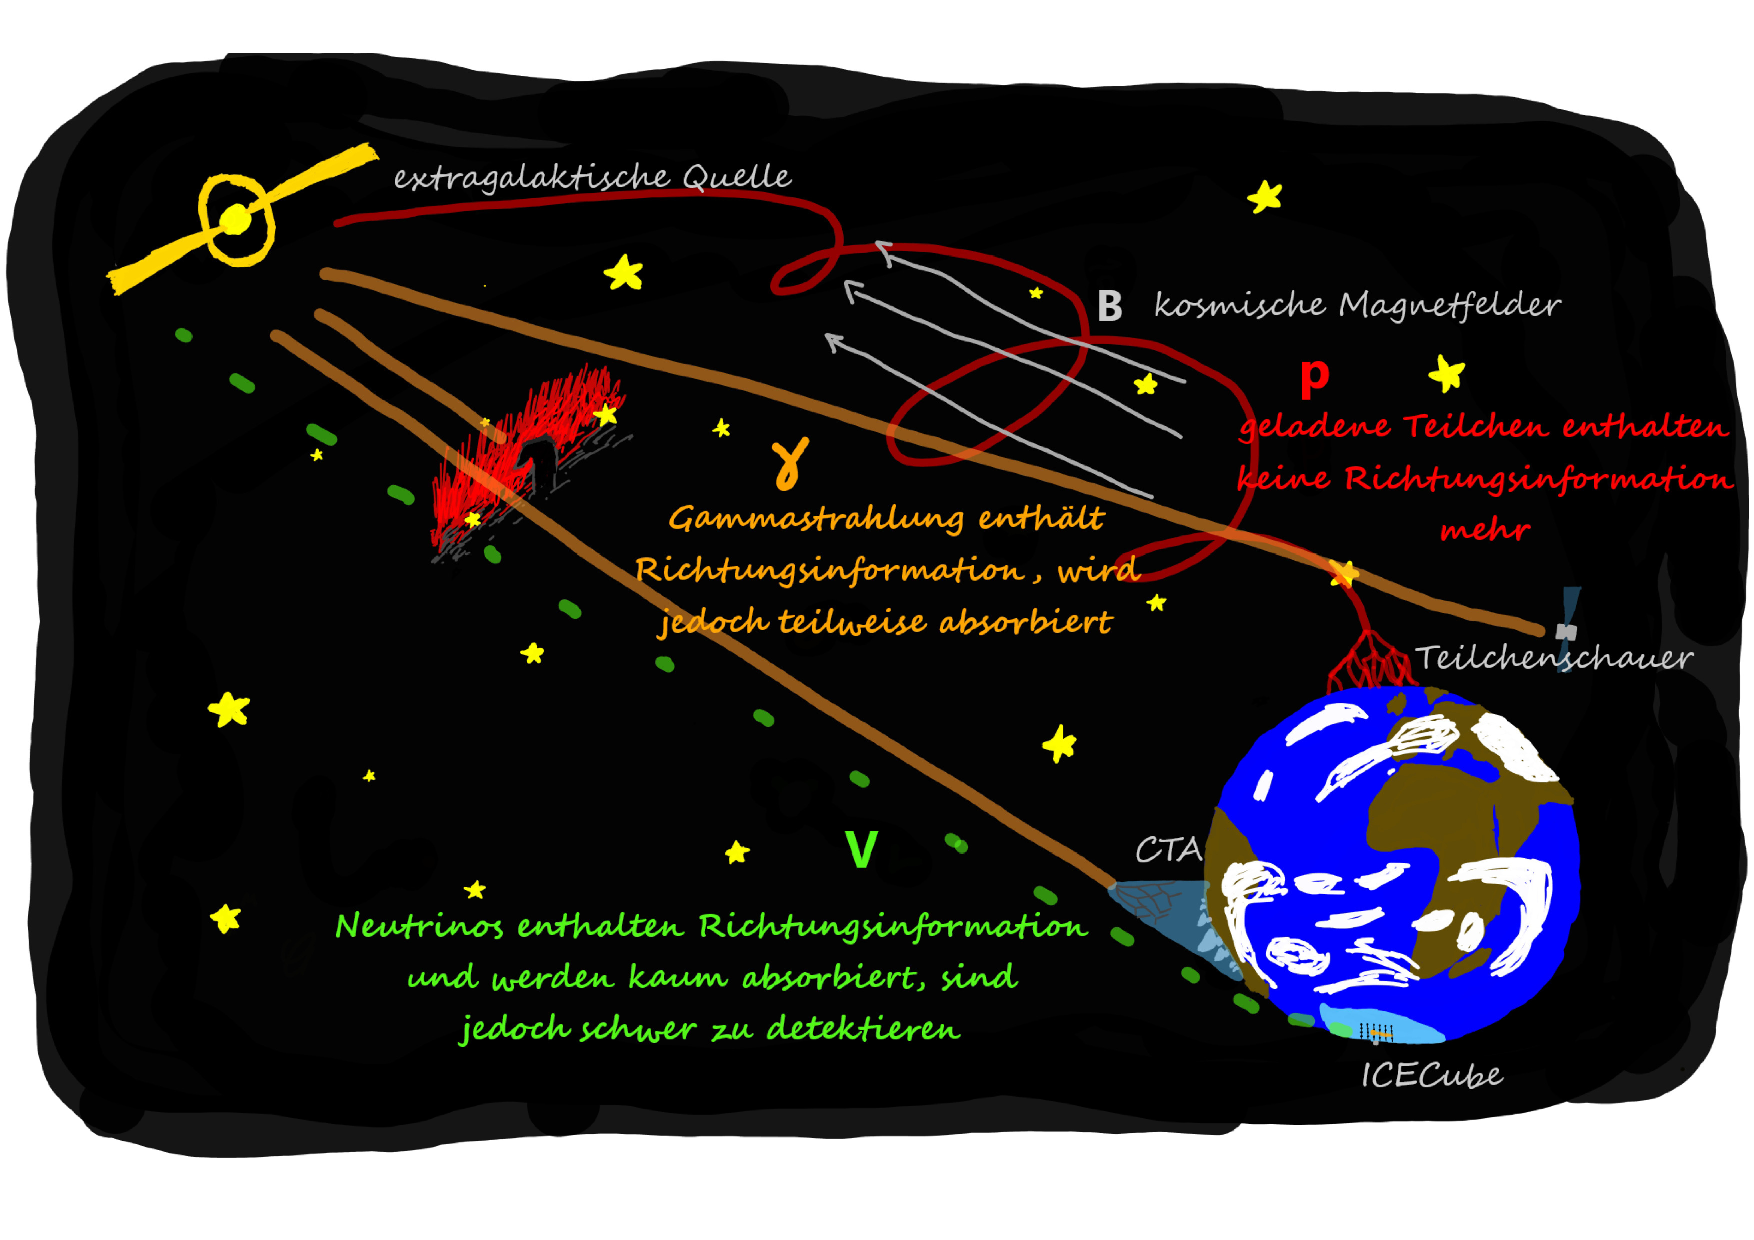
\includegraphics[width=0.7\textwidth]{pictures/Folie5.pdf}
        \caption{}
        \label{abb:folie5}
      \end{figure}
  \end{frame}


  \begin{frame}
    \frametitle{Funtionsweise von CTA}
    \begin{columns}
      \column{0.6\textwidth}
        \begin{figure}
          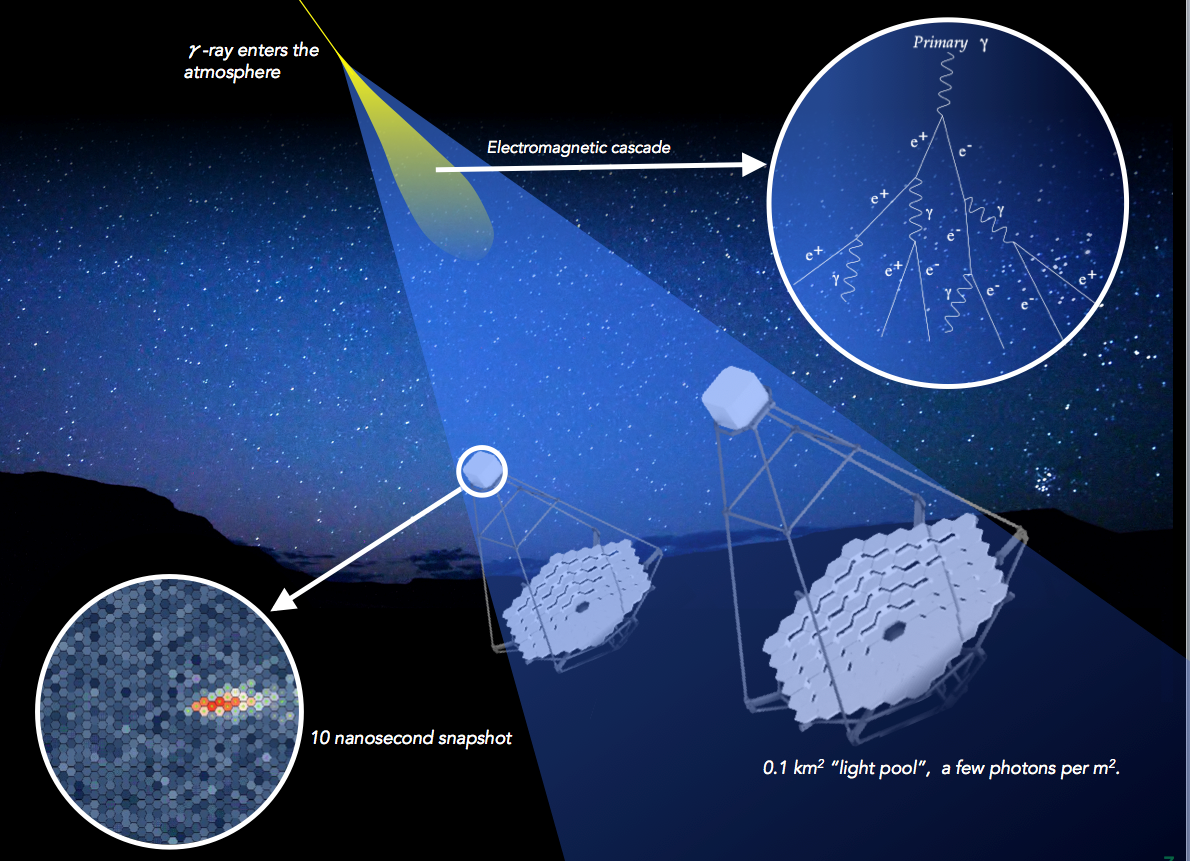
\includegraphics[width=0.95\textwidth]{pictures/CTA.png}
          \caption{CTA hompage (How CTA works)}
          \label{abb:CTA}
        \end{figure}
      \column{0.4\textwidth}
        \begin{itemize}
          \item Photon wechselwirkt mit der Atmosphäre: Schauer entsteht
          \item Lichtgeschwindigkeit in Atmosphäre $\SI{0.03}{\percent}$ langsamer als Vakuum.
          \item Überlichtschnelle geladene Teilchen senden Kegel aus Cherenkov-Licht aus.
          \item Durchmesser: $\SI{250}{\m}$
          \item Dauer: einige $\si{\nano\s}$.
        \end{itemize}
    \end{columns}
  \end{frame}
  \begin{frame}
    \frametitle{Information über das Schauer}
    \begin{columns}
      \column{0.4\textwidth}
        \begin{itemize}
          \item Hillas Parameter, Wölbung und Krümmung
          \item Scaled Cuts Technik: $SV = \frac{v- \langle v \rangle}{\sigma_v}$ für $v=w\text{;}l$~\cite[104]{SV}
          \item Teleskop-Typ
          \item Anzahl der ausgelösten Teleskope, LST, MST und SST
          \item gesamte Intensität
          \item Art des Primärteilchens
        \end{itemize}
      \column{0.6\textwidth}
        \begin{figure}
          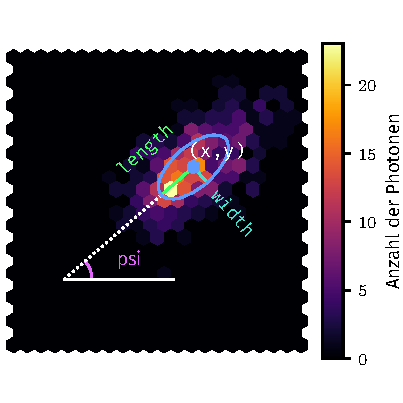
\includegraphics[width=0.7\textwidth]{pictures/hillas_2.pdf}
          \caption{Max Nöthe}
          \label{abb:Hillas}
        \end{figure}
    \end{columns}
  \end{frame}

  \begin{frame}
    \frametitle{Aufgabenspektrum}
    \begin{itemize}
      \item Entdecken neuer glaktischer Gammaquellen (SNR, PWN, Doppelsysteme, galaktische Zentrum)
      \item Multiwellenlängen- und Multimessenger-Beobachtungen um hadronische Beschleunigungsprozesse zu Untersuchen
      \item Entdecken neuer Quellen mit großer Rotverschiebung
      \item Detektieren von Zerfällen der Dunklen Materie
      \item \dots
    \end{itemize}
  \end{frame}


  \subsection{Maschinelles Lernen}

  \begin{frame}
    \frametitle{Entscheidungsbaum}
    \begin{columns}
      \column{0.7\textwidth}
      \begin{figure}
        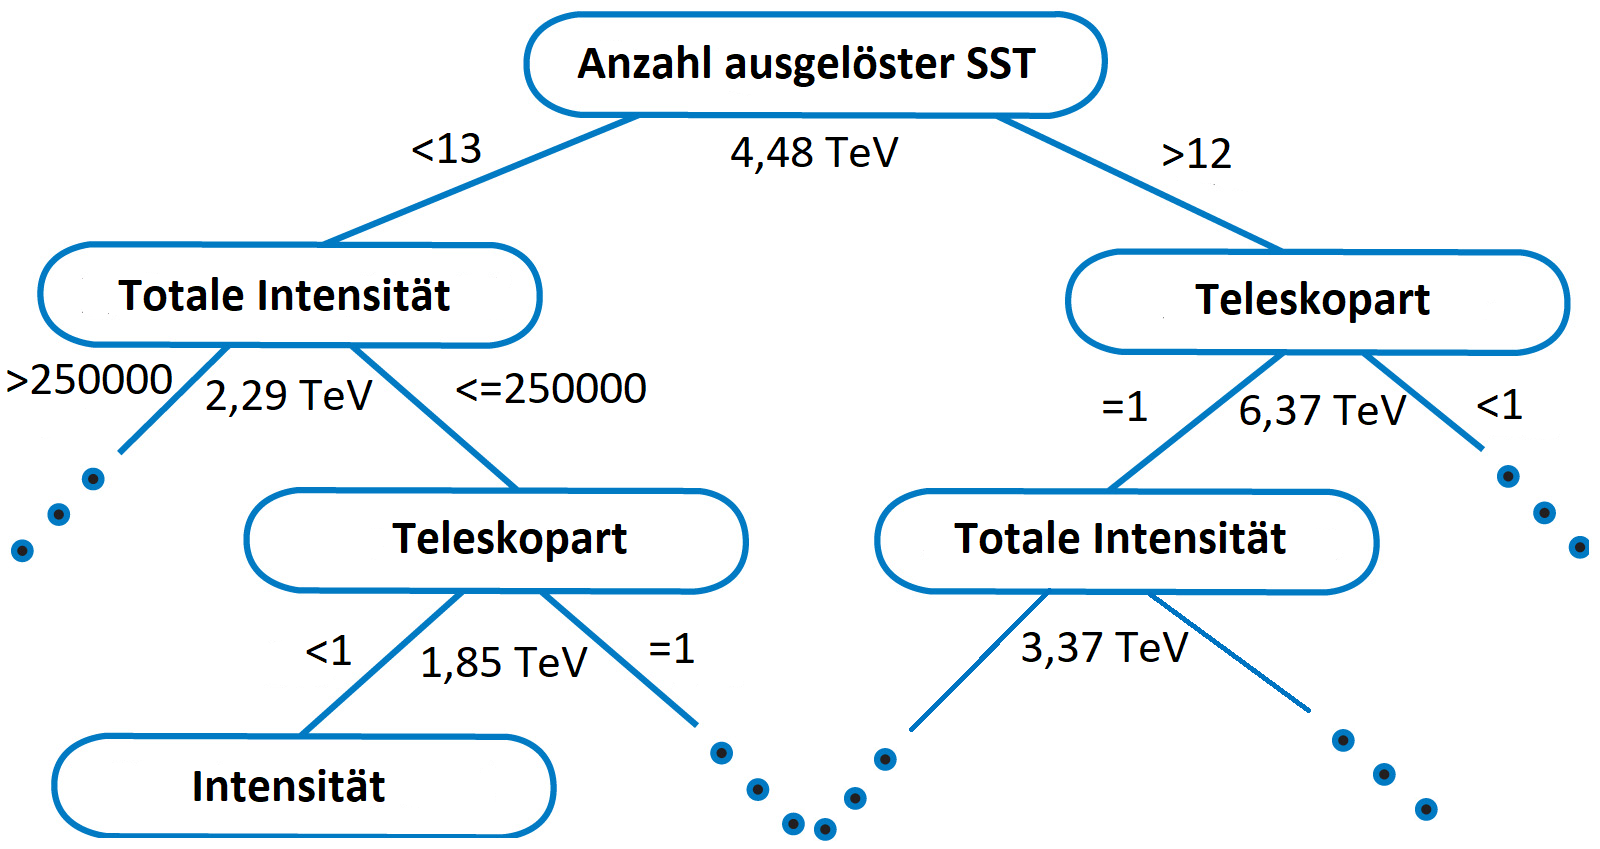
\includegraphics[width=0.8\textwidth]{pictures/Decisiontree.png}
        \caption{}
        \label{abb:DT}
      \end{figure}
      \column{0.3\textwidth}
      \begin{block}{Kriterium}
        \begin{equation*}
          \symbf{H}(\symbf{X}_m) = \frac{1}{N_m}\sum_{i\in N_m}(\symbf{\hat{y}}_i-\symbf{c}_m)^2
        \end{equation*}
        mit
        \begin{equation*}
          \symbf{c}_m = \frac{1}{N_m}\sum_{i\in N_m}\symbf{\hat{y}}_i
        \end{equation*}
      \end{block}
    \end{columns}

  \end{frame}
  \begin{frame}
    \frametitle{Random Forest}
    \begin{columns}
      \column{0.6\textwidth}
      \begin{figure}
        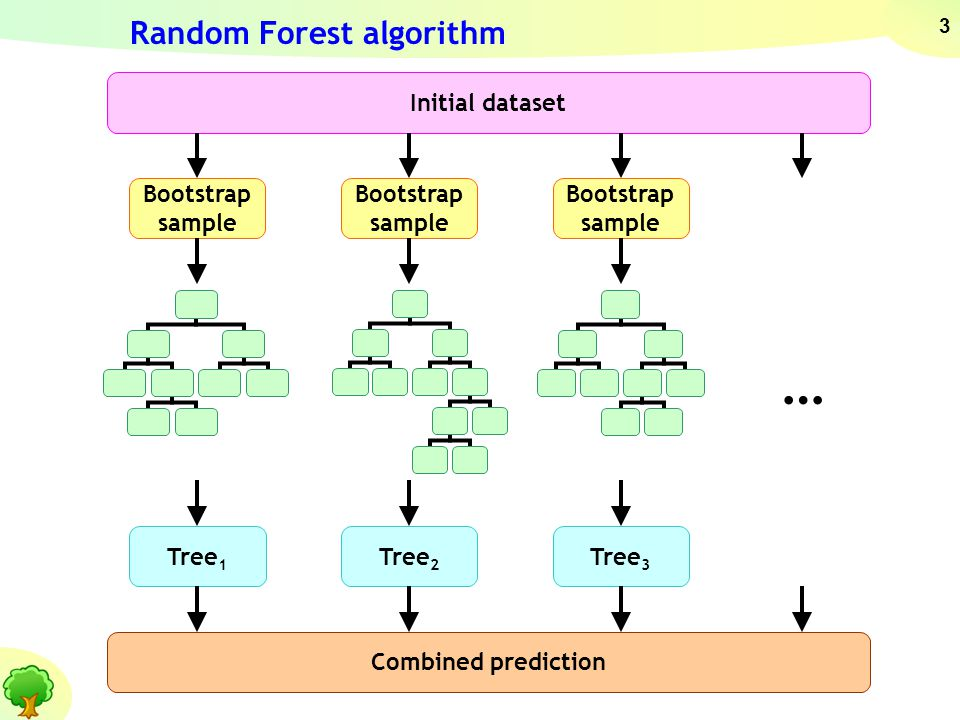
\includegraphics[width=0.9\textwidth]{pictures/RF.jpg}
        \caption{Pavel Polishchuk}
        \label{abb:RF}
      \end{figure}
      \column{0.4\textwidth}
      Warum der Random Forest Algorithmus:
      \begin{itemize}
        \item Interpretierbarkeit
        \item Zeitkomplexität: $\Omega(n\log(n))$
        \item einfache Datenpräparation
        \item nicht anfällig gegen unbedeutende Attribute
        \item Stabiles Ergebnis
      \end{itemize}
    \end{columns}
  \end{frame}

  \section{Ergebnisse}
  \subsection{Rekonstruktion mit RF Regressor}

  \begin{frame}
    \frametitle{Energierekonstruktion mit dem Random Forest}
    \begin{figure}
      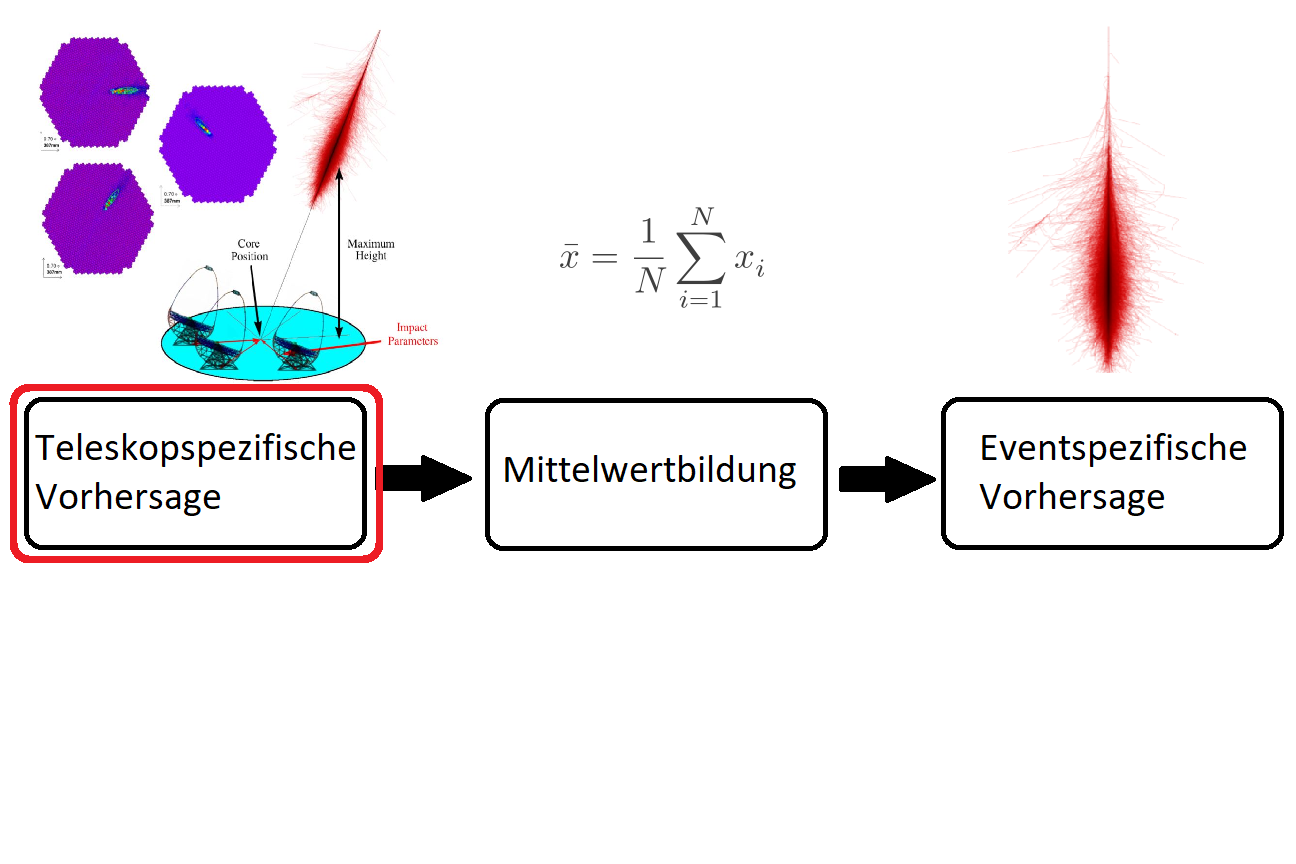
\includegraphics[width=\textwidth]{pictures/Ablauf10.png}
      \caption{}
      \label{}
    \end{figure}
  \end{frame}

  \begin{frame}
    \frametitle{Schätzung jedes Teleskop-Ereignis}
    \begin{columns}
      \column{0.5\textwidth}
        \begin{itemize}
          \item Datensatz:
            \begin{itemize}
              \item $\num{3322938}$ Teleskop-Events
              \item $\num{996653}$ Array-Events
              \item $\SI{78}{\percent}$ punktgerichtet und $\SI{22}{\percent}$ diffuse
              \item $\SI{33}{\percent}$ Trainings- und $\SI{66}{\percent}$ Testdatensatz
            \end{itemize}
          \item Random Forest:
            \begin{itemize}
              \item maximale Tiefe $=\num{10}$
              \item Größe des Waldes $=\num{100}$
              \item Anzahl der Attribute $=\sqrt{N}$
              \item Minimale Blattgröße $=\num{1}$
            \end{itemize}
          \item $R^2$-Score:
          \begin{equation*}
            R^2 = 1 - \frac{\sum_i (y_i-\hat{y}_i)^2}{\sum_i (y_i - \overline{y})^2}
          \end{equation*}
        \end{itemize}
      \column{0.5\textwidth}
      \begin{figure}
        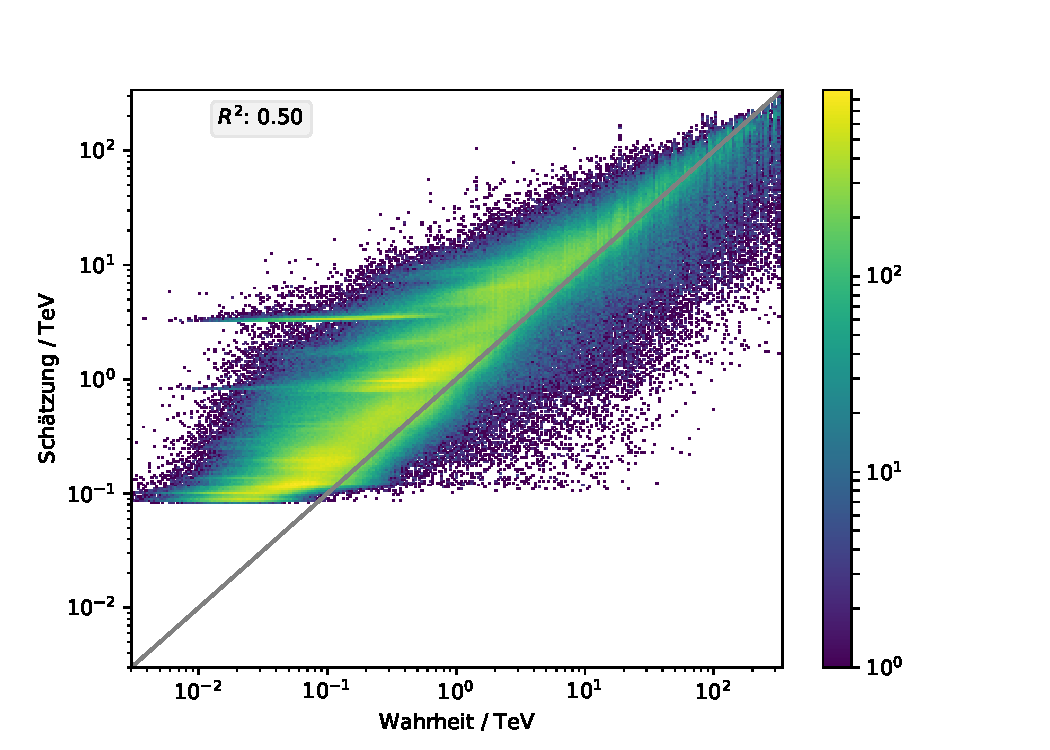
\includegraphics[width=1.1\textwidth]{pictures/RF.pdf}
        \caption{}
        \label{}
      \end{figure}
    \end{columns}
  \end{frame}

  \begin{frame}
    \frametitle{Rangliste der Attribute}
    \begin{columns}
      \column{0.6\textwidth}
      \begin{figure}
        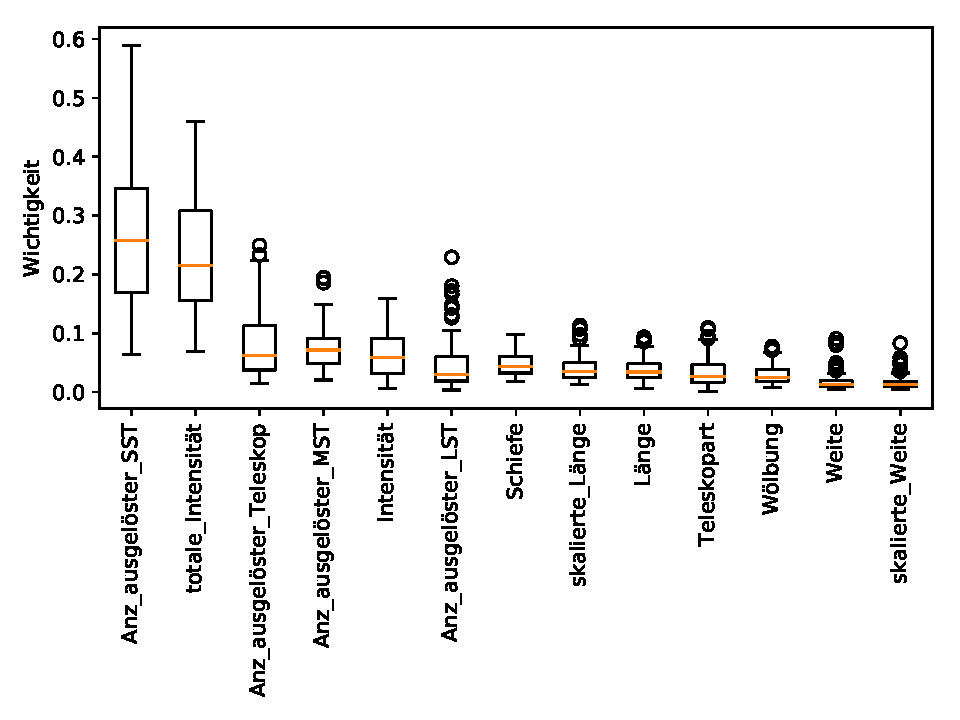
\includegraphics[width=\textwidth]{pictures/feautureimportance_boxplot_firstForest.pdf}
        \caption{}
        \label{}
      \end{figure}
      \column{0.4\textwidth}
      \begin{block}{Kriterium}
        Rangordnung der Attribute in jedem Entscheidungsbaum
      \end{block}
      \begin{itemize}
        \item Aufgrund von Bootstrapping und dem CART-Algorithmus kann eine Verzerrung auftreten
        \item Attribute mit einer kleinen Anzahl an Kategorien werden unterschätzt
      \end{itemize}
    \end{columns}
  \end{frame}

  \subsection{Optimierung durch Mittelwert}

  \begin{frame}
    \frametitle{Energierekonstruktion mit dem Random Forest}
    \begin{figure}
      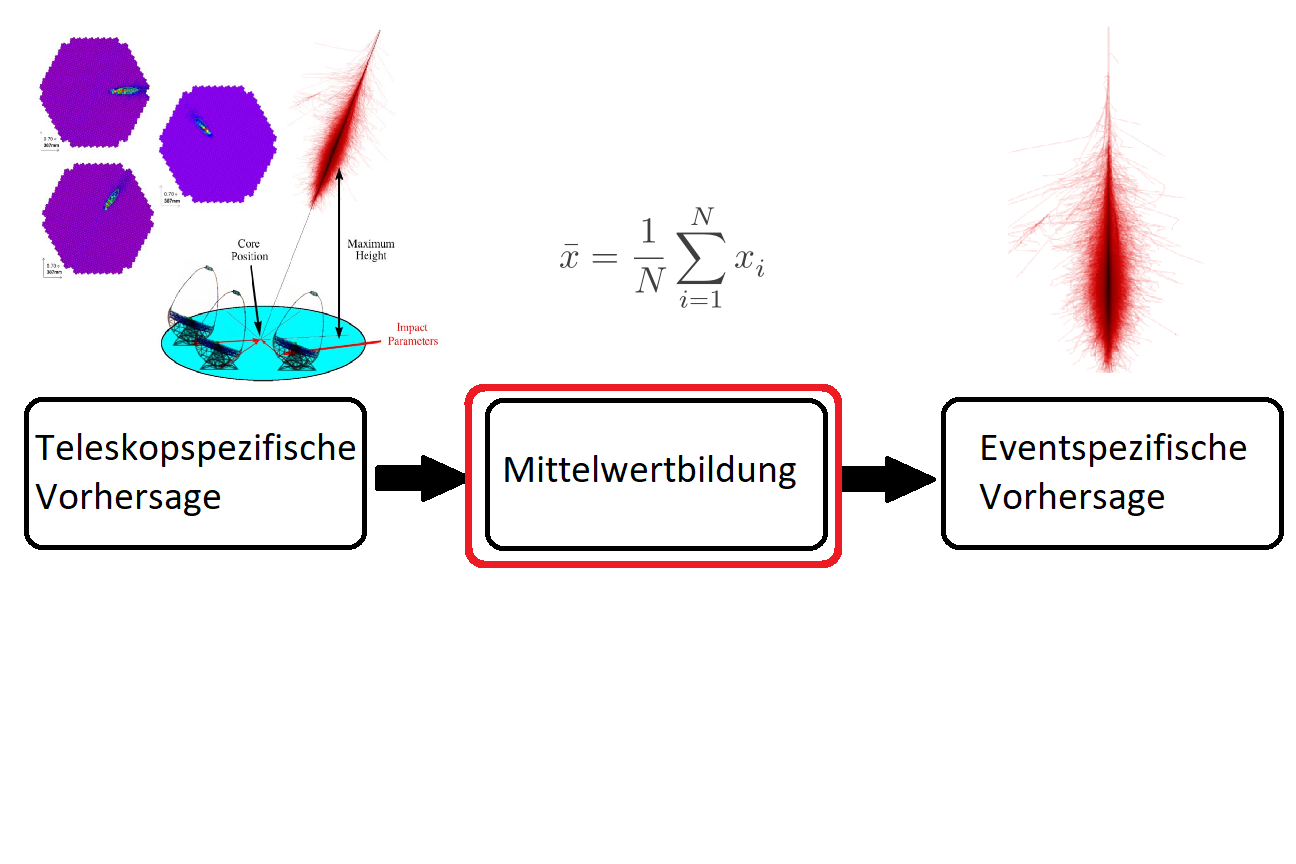
\includegraphics[width=\textwidth]{pictures/Ablauf11.png}
      \caption{}
      \label{}
    \end{figure}
  \end{frame}

  \begin{frame}
    \frametitle{Arithmetisches Mittel und Median}
    \begin{columns}
      \column{0.5\textwidth}
      \begin{figure}
        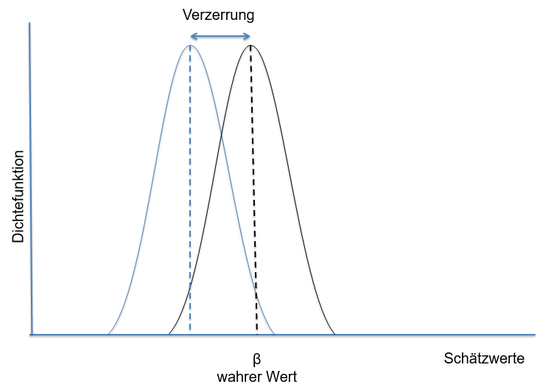
\includegraphics[width=\textwidth]{pictures/Bias.png}
        \caption{}
        \label{}
      \end{figure}
      \column{0.5\textwidth}
      \begin{figure}
        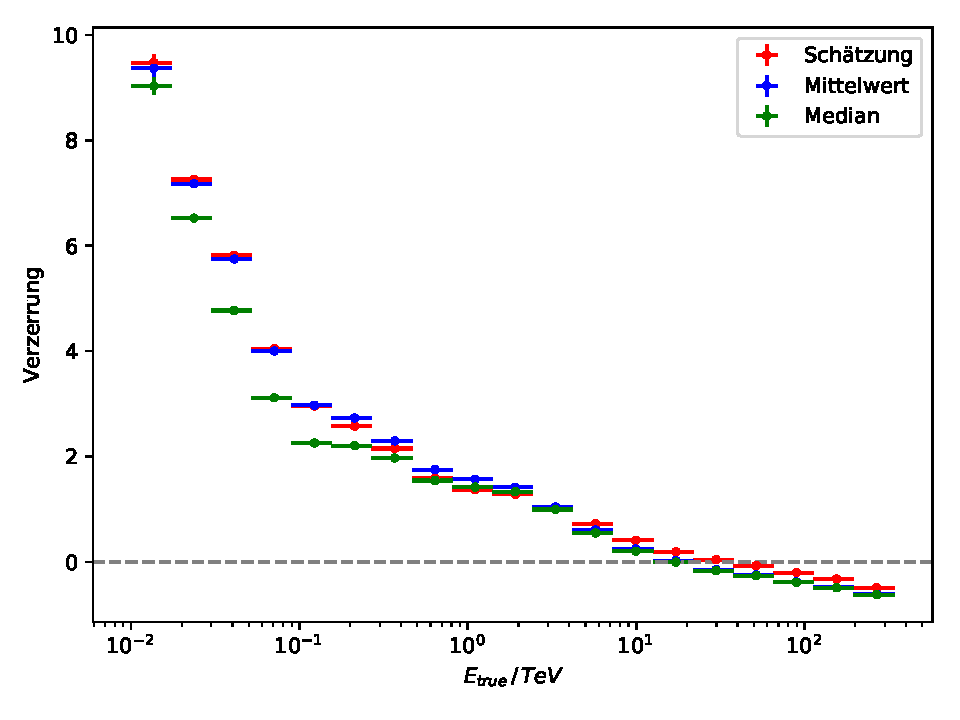
\includegraphics[width=\textwidth]{pictures/RF_mean_bias.pdf}
        \caption{Mittelwert des relativen Fehlers für verschiedene Energiebereiche.}
        \label{}
      \end{figure}
    \end{columns}
  \end{frame}

  \begin{frame}
    \begin{columns}
      \column{0.5\textwidth}
      \begin{figure}
        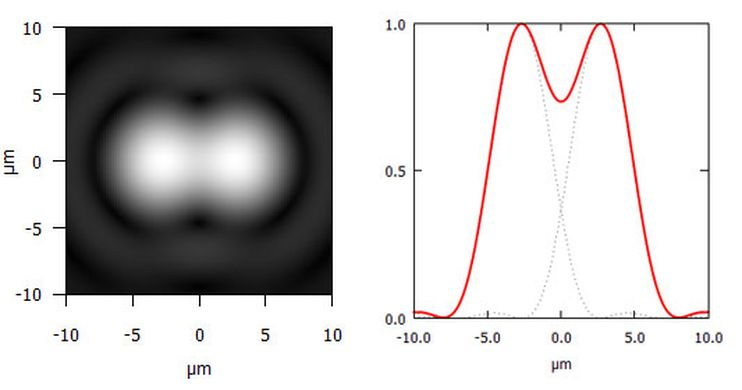
\includegraphics[width=\textwidth]{pictures/resolution.jpg}
        \caption{}
        \label{}
      \end{figure}
      \column{0.5\textwidth}
      \begin{figure}
        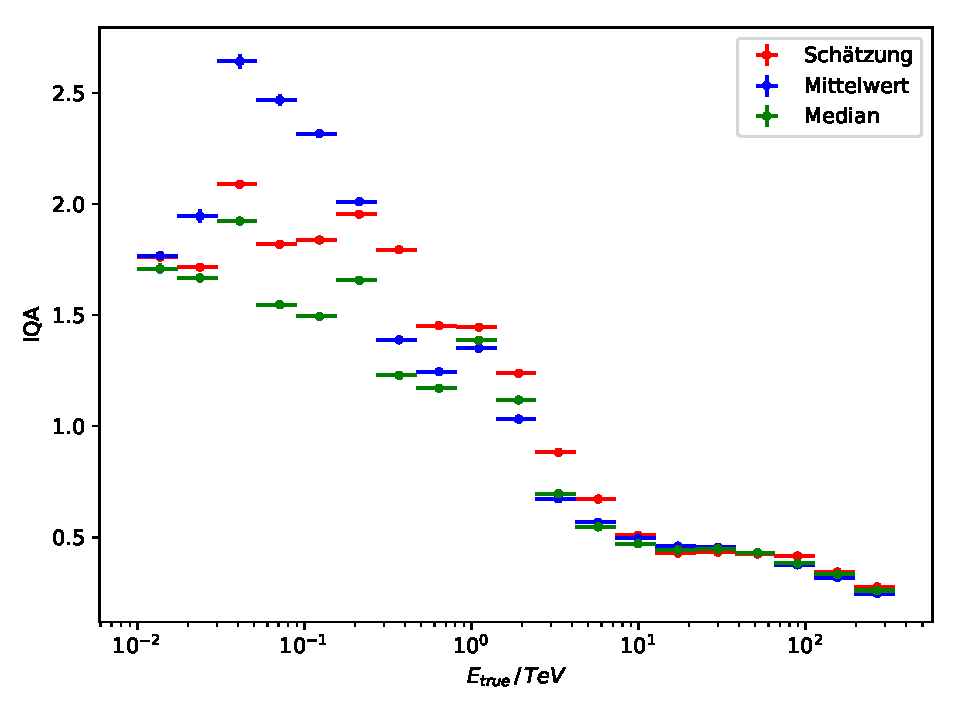
\includegraphics[width=\textwidth]{pictures/RF_mean_resolution.pdf}
        \caption{Die Hälfte des IQA von $\SI{68,26}{\percent}$ des relativen Fehlers für verschiedene Energiebereiche.}
        \label{}
      \end{figure}
    \end{columns}
  \end{frame}

  \begin{frame}
    \begin{columns}
      \column{0.5\textwidth}
      \begin{figure}
        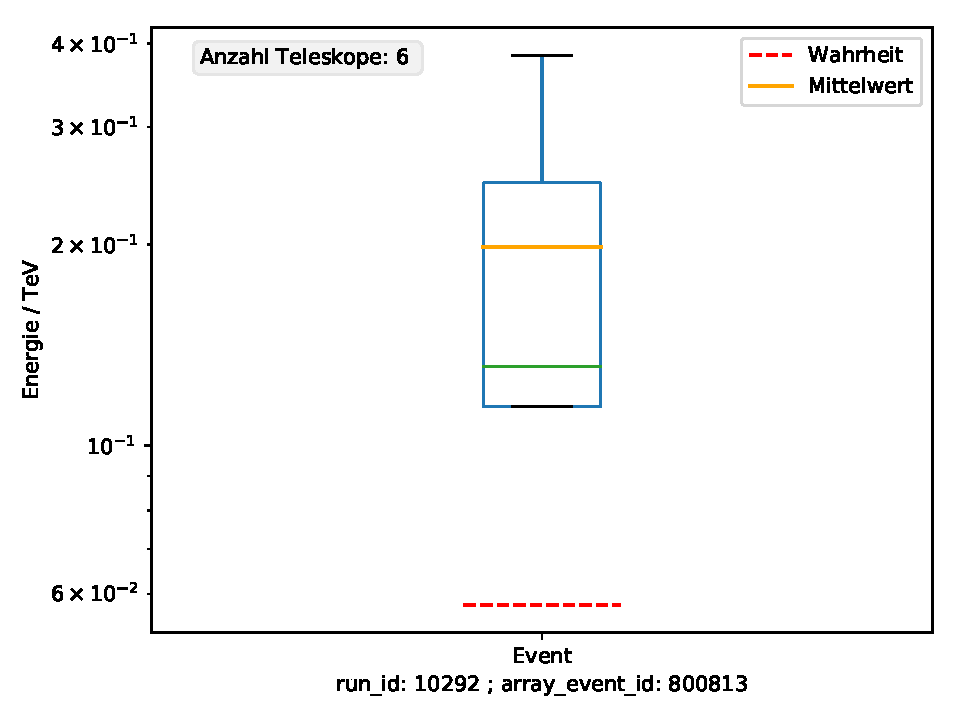
\includegraphics[width=\textwidth]{pictures/pred2.pdf}
        \caption{Zufällige Vorhersage für das Array-Event:}
        \label{}
      \end{figure}
      \column{0.5\textwidth}
      \begin{figure}
        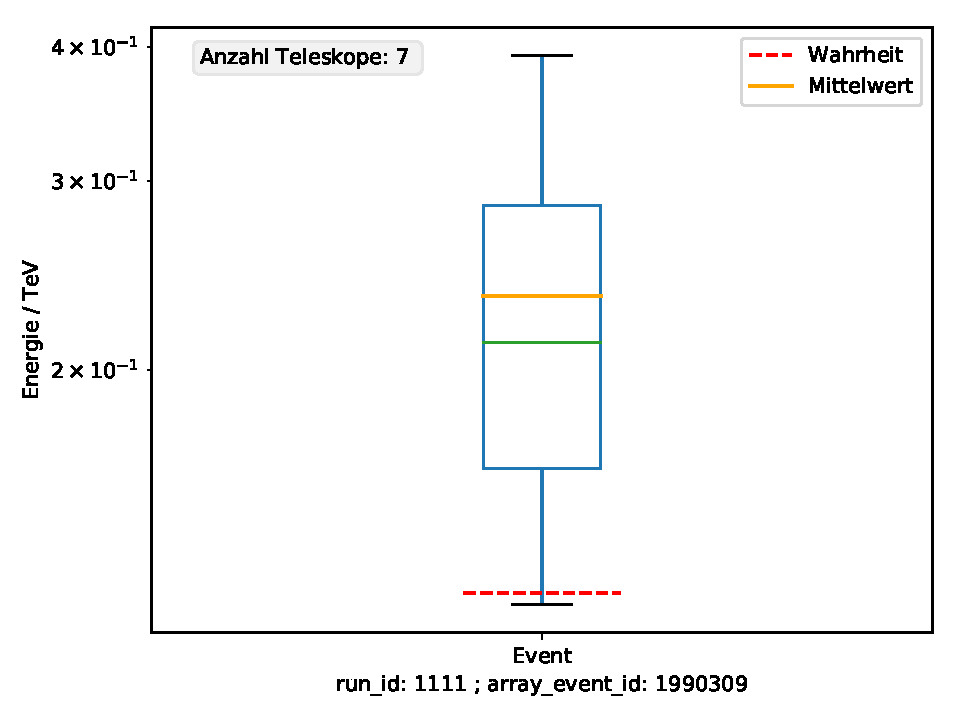
\includegraphics[width=\textwidth]{pictures/pred3.pdf}
        \caption{Zufällige Vorhersage für das Array-Event:}
        \label{}
      \end{figure}
    \end{columns}
  \end{frame}

  \begin{frame}
    \frametitle{Intensität als Gewicht}
    \begin{figure}
      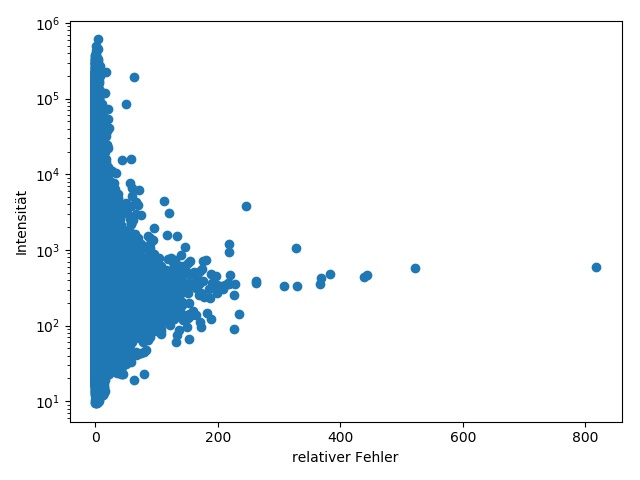
\includegraphics[width=0.5\textwidth]{pictures/intensity.jpg}
      \caption{}
      \label{}
    \end{figure}
  \end{frame}

  \begin{frame}
    \frametitle{Sensitivität als Gewicht}
    \begin{figure}
      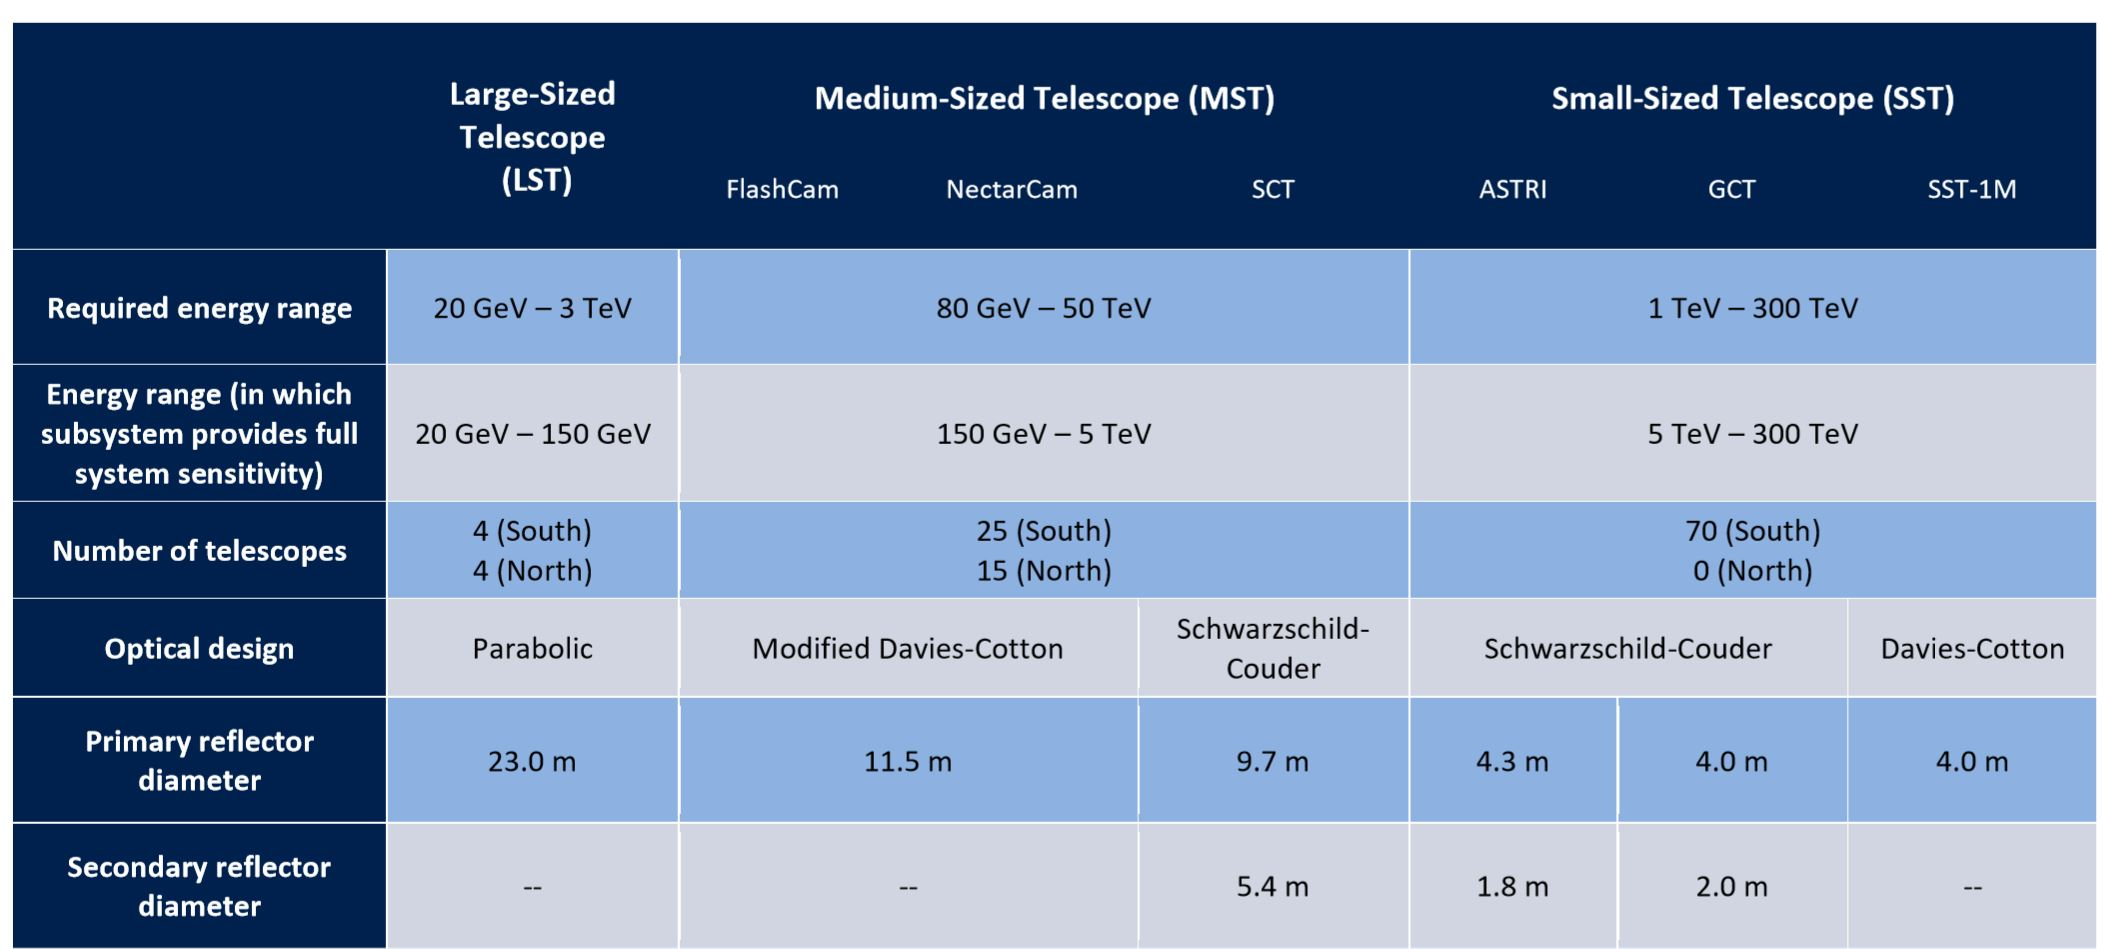
\includegraphics[width=0.7\textwidth]{pictures/Spec.JPG}
      \caption{CTA homepage (CTA technology)}
      \label{}
    \end{figure}
    \begin{columns}
      \column{0.33\textwidth}
      Vollsensitiver Bereich: $\num{2}$
      \column{0.33\textwidth}
      Teilsensitiver Bereich: $\num{1}$
      \column{0.33\textwidth}
       Außerhalb der Bereiche: $\num{0.1}$
    \end{columns}
  \end{frame}

  \begin{frame}
    \begin{columns}
      \column{0.5\textwidth}
      \begin{figure}
        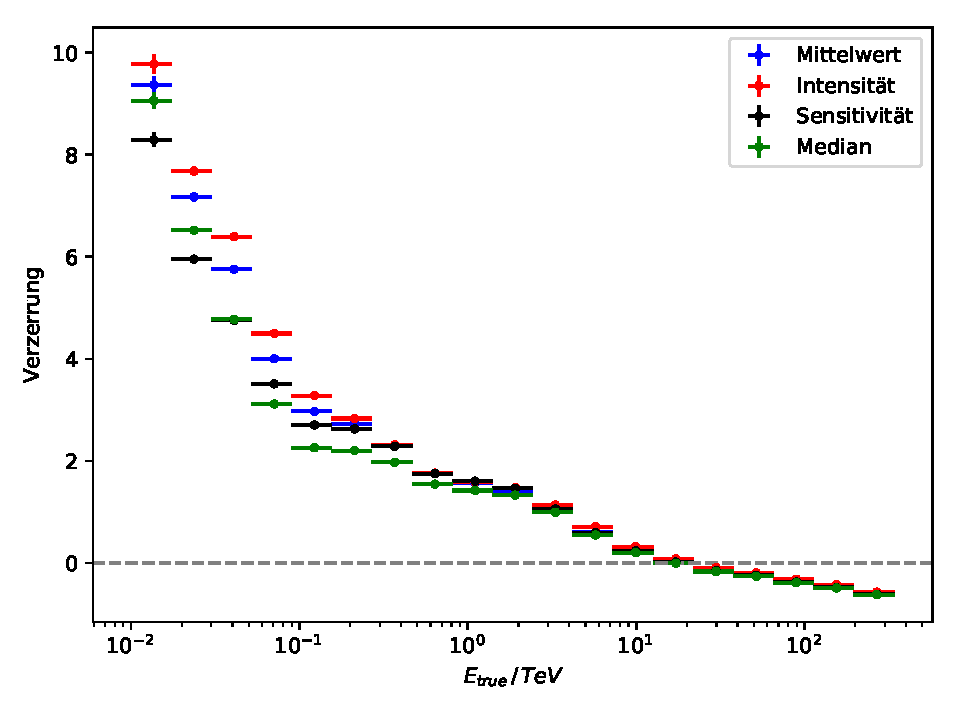
\includegraphics[width=\textwidth]{pictures/RF_weights_bias.pdf}
        \caption{Mittelwert des relativen Fehlers für verschiedene Energiebereiche.}
        \label{}
      \end{figure}
      \column{0.5\textwidth}
      \begin{figure}
        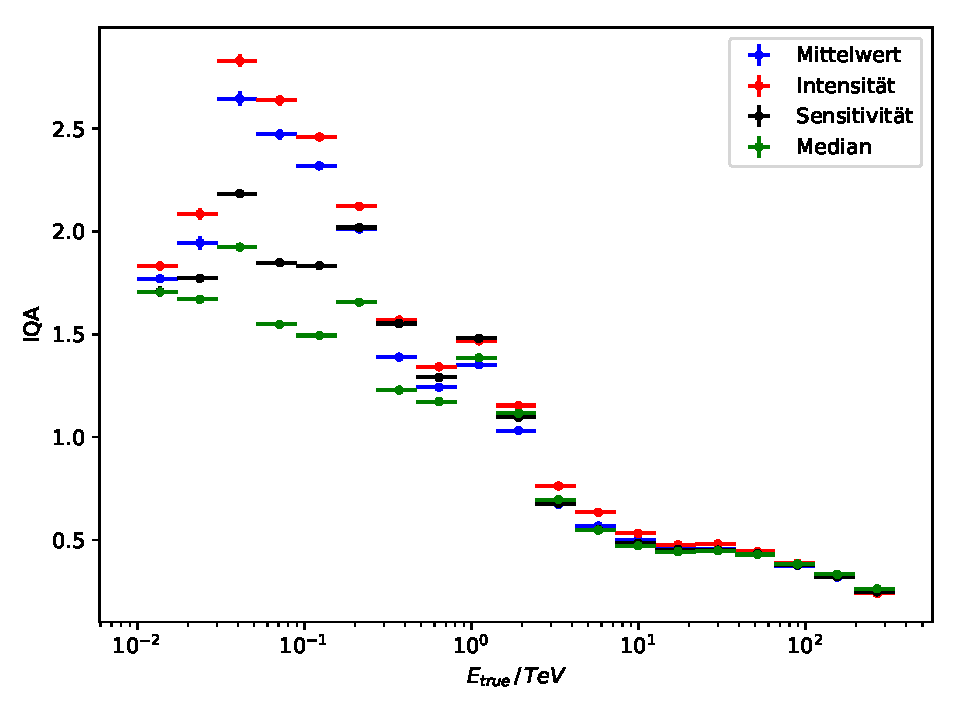
\includegraphics[width=\textwidth]{pictures/RF_weights_resolution.pdf}
        \caption{Die Hälfte des IQA von $\SI{68,26}{\percent}$ des relativen Fehlers für verschiedene Energiebereiche.}
        \label{}
      \end{figure}
    \end{columns}
  \end{frame}

  \subsection{Verschachtelte Methode}

  \begin{frame}
    \frametitle{Energierekonstruktion mit dem Random Forest}
    \begin{figure}
      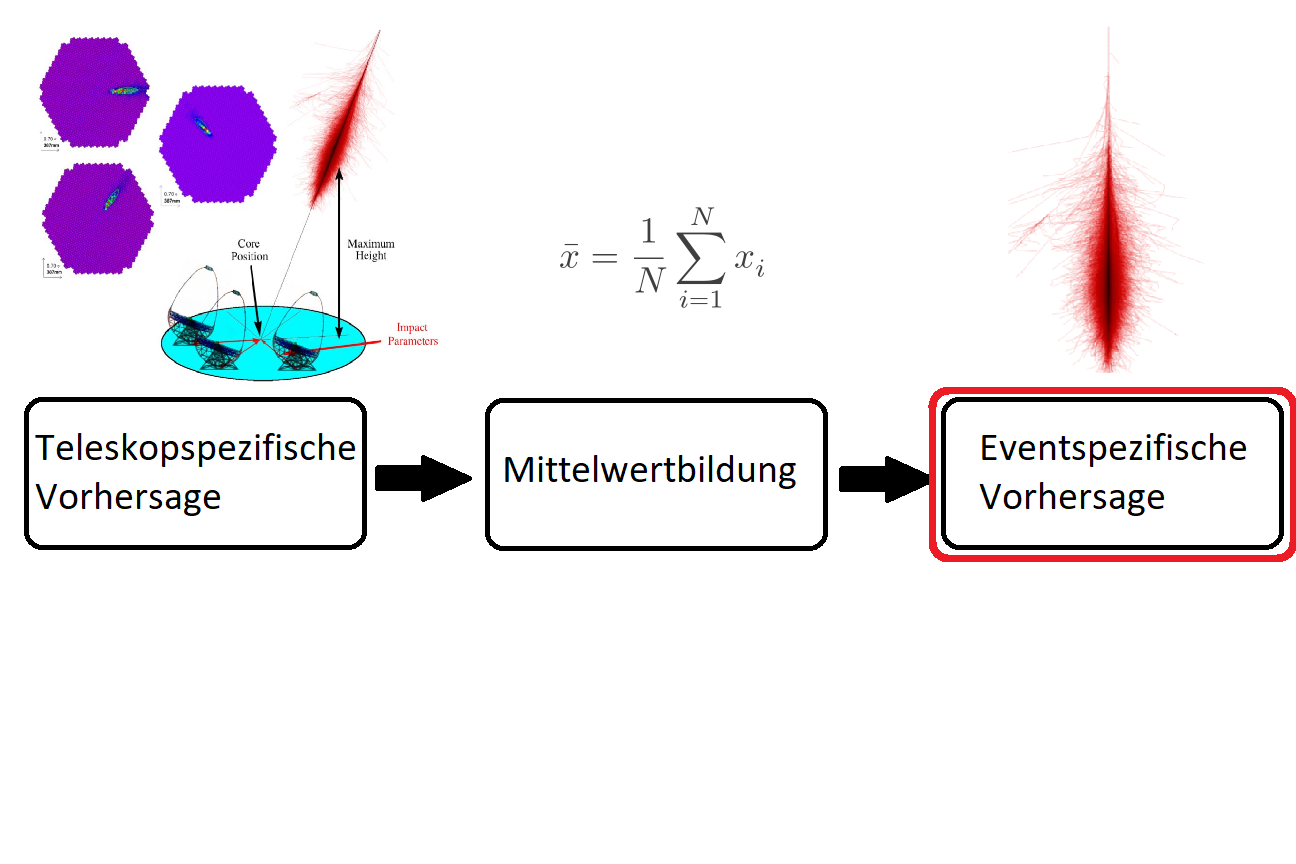
\includegraphics[width=\textwidth]{pictures/Ablauf12.png}
      \caption{}
      \label{}
    \end{figure}
  \end{frame}

  \begin{frame}
    \frametitle{Eventspezifische Vorhersage}
    \begin{columns}
      \column{0.5\textwidth}
      \begin{itemize}
        \item Attribute:
        \begin{itemize}
          \item totale Intensität, Anzahl ausgelöster Teleskope, SST, MST, LST
          \item Mittelwert und Standardabweichung der skalierten Größen
          \item Mittelwert der vorherigen Schätzungen
          \item Mittelwert, Standardabweichung, Maximum und Minimum der Schätzungen der SST, MST und LST
        \end{itemize}
        \item Parameter des Random Forest sind die gleichen
        \item Datensatz
        \begin{itemize}
          \item Traingsdatensatz: $\num{498146}$
          \item Testdatensatz: $\num{498507}$
        \end{itemize}
      \end{itemize}
      \column{0.5\textwidth}
      \begin{figure}
        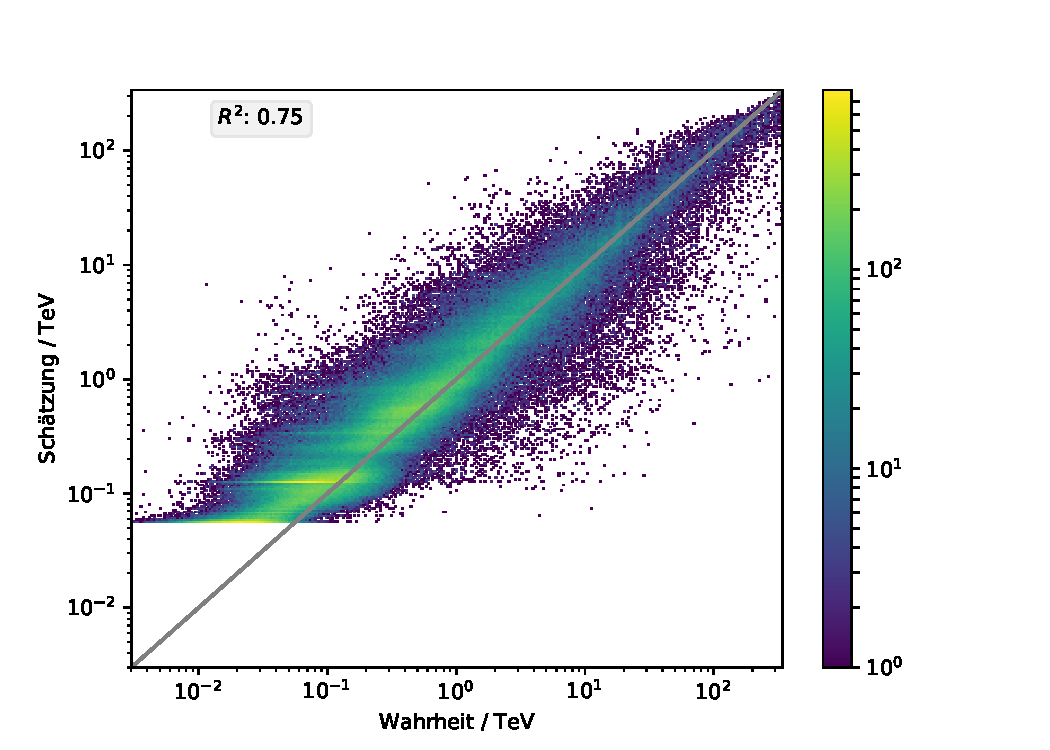
\includegraphics[width=1.1\textwidth]{pictures/RF_encaps.pdf}
        \caption{}
        \label{}
      \end{figure}
    \end{columns}
  \end{frame}

  \begin{frame}
    \frametitle{Rangsliste der Attribute des zweiten Random Forest}
    \begin{figure}
      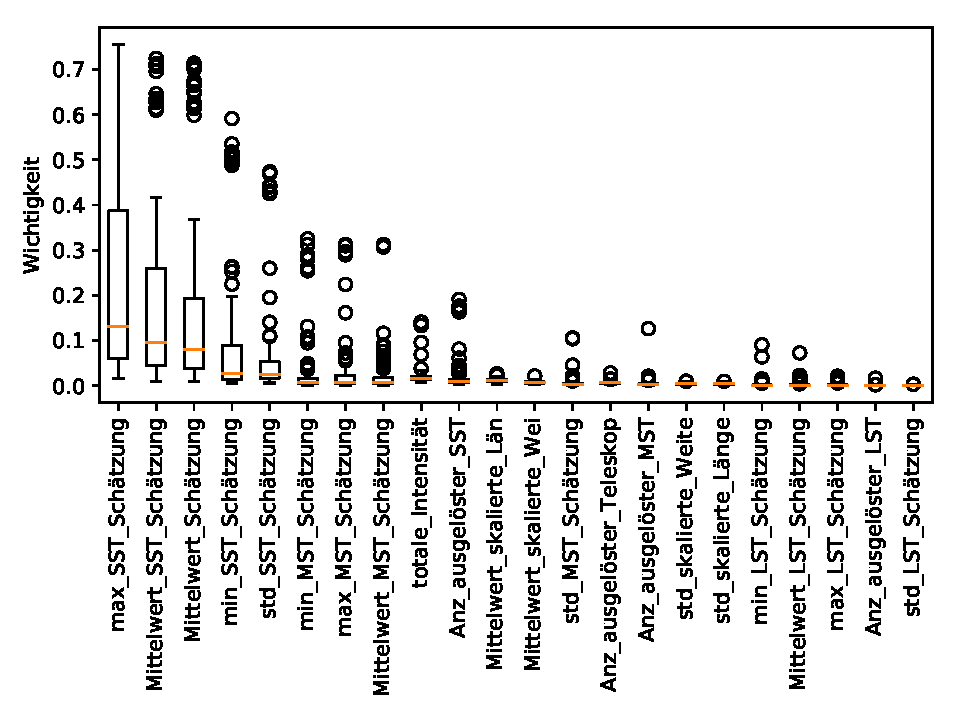
\includegraphics[width=0.55\textwidth]{pictures/feautureimportance_boxplot_secondForest.pdf}
      \caption{}
      \label{}
    \end{figure}
  \end{frame}

  \begin{frame}
    \begin{columns}
      \column{0.5\textwidth}
      \begin{figure}
        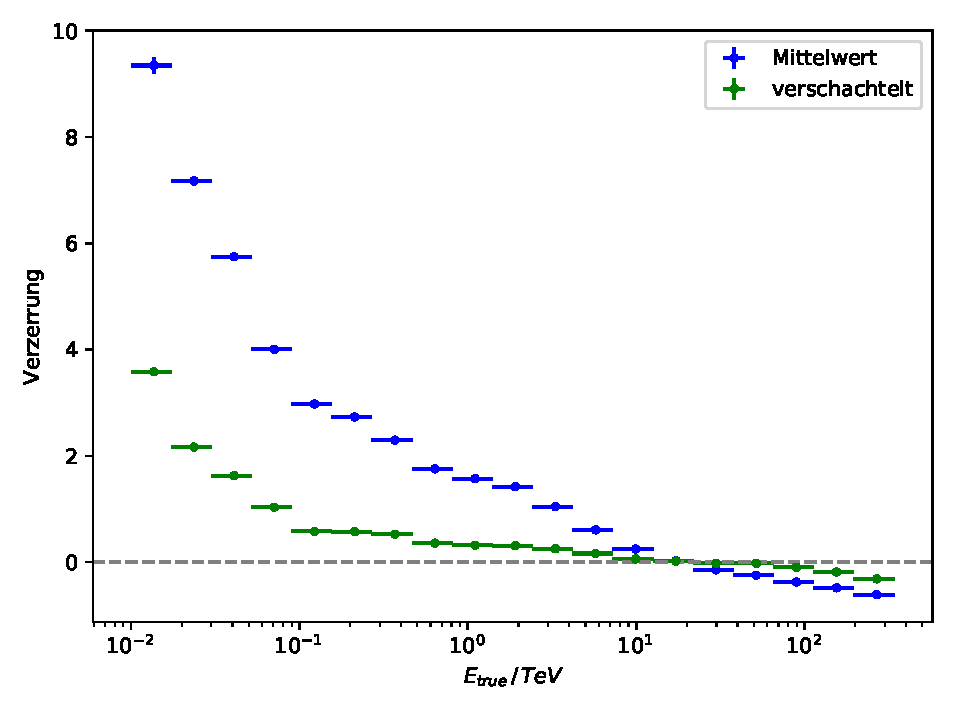
\includegraphics[width=\textwidth]{pictures/RF_nested_bias.pdf}
        \caption{Mittelwert des relativen Fehlers für verschiedene Energiebereiche.}
        \label{}
      \end{figure}
      \column{0.5\textwidth}
      \begin{figure}
        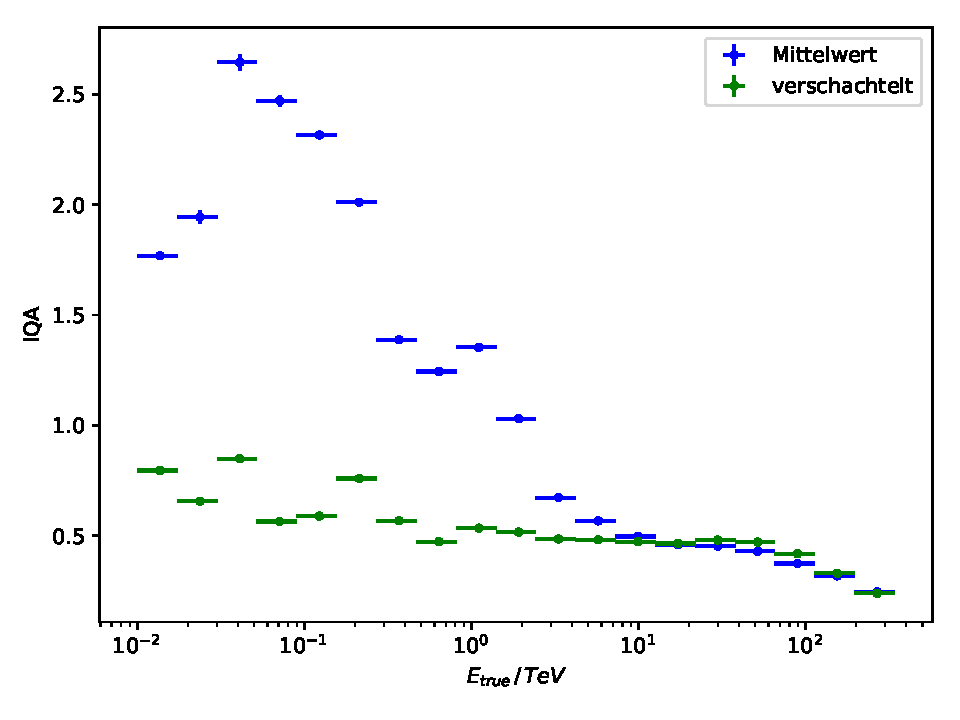
\includegraphics[width=\textwidth]{pictures/RF_nested_resolution.pdf}
        \caption{Die Hälfte des IQA von $\SI{68,26}{\percent}$ des relativen Fehlers für verschiedene Energiebereiche.}
        \label{}
      \end{figure}
    \end{columns}
  \end{frame}

  \subsection{Energie-Transformation}

  \begin{frame}
    \frametitle{Transformation der Energien}
    \begin{figure}
      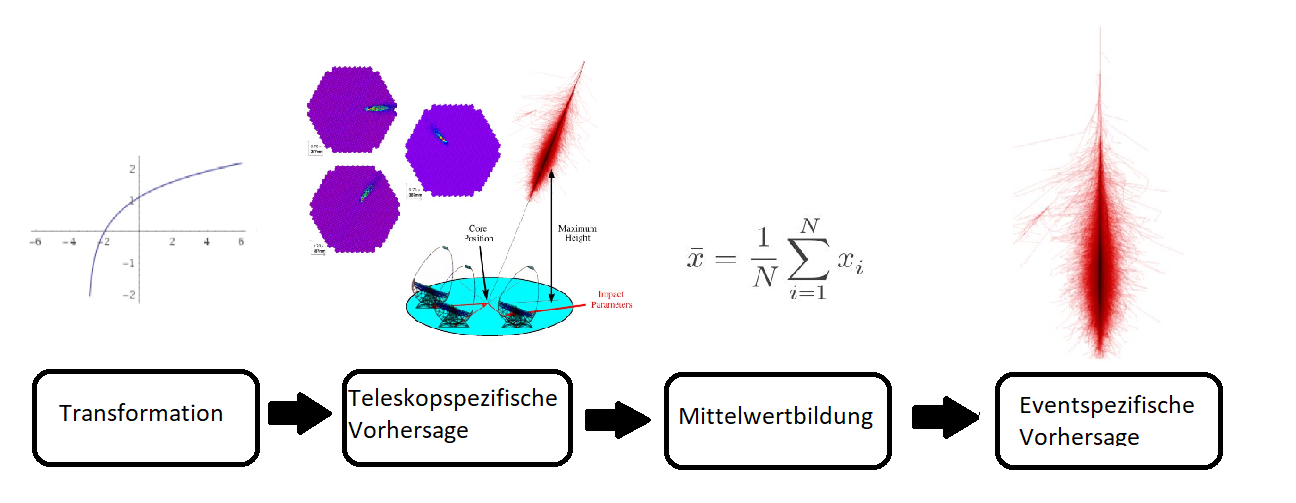
\includegraphics[width=0.6\textwidth]{pictures/Ablauf2.png}
      \caption{}
      \label{}
    \end{figure}
    \begin{columns}
      \column{0.5\textwidth}
      Bijektive Transformation auf $\symbb{R}^+$:
      \begin{equation*}
        E_{\symup{trafo}}=\ln(E_\gamma +3)
        \label{eqn:trafo}
      \end{equation*}
      \column{0.5\textwidth}
      Rücktransformation:
      \begin{equation*}
        E_\gamma = \exp \left(E_{\symup{trafo}}\right)-3
      \end{equation*}
    \end{columns}
  \end{frame}

  \begin{frame}
    \begin{columns}
      \column{0.5\textwidth}
      \begin{figure}
        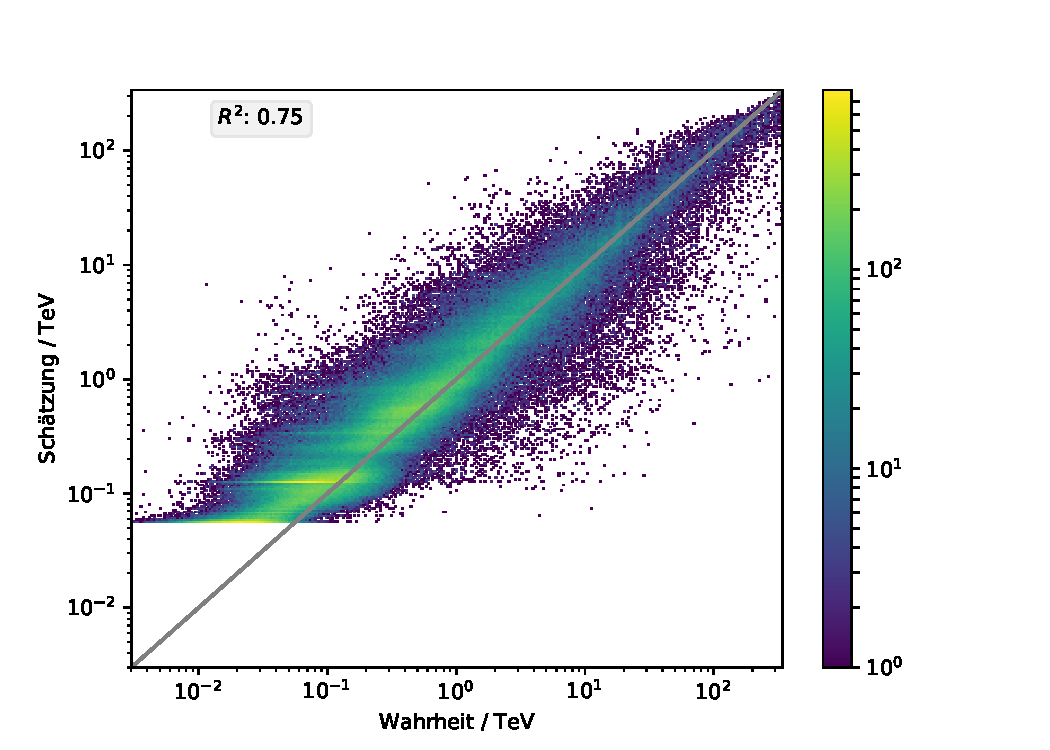
\includegraphics[width=1.1\textwidth]{pictures/RF_encaps.pdf}
        \caption{Ohne Transformation}
        \label{}
      \end{figure}
      \column{0.5\textwidth}
      \begin{figure}
        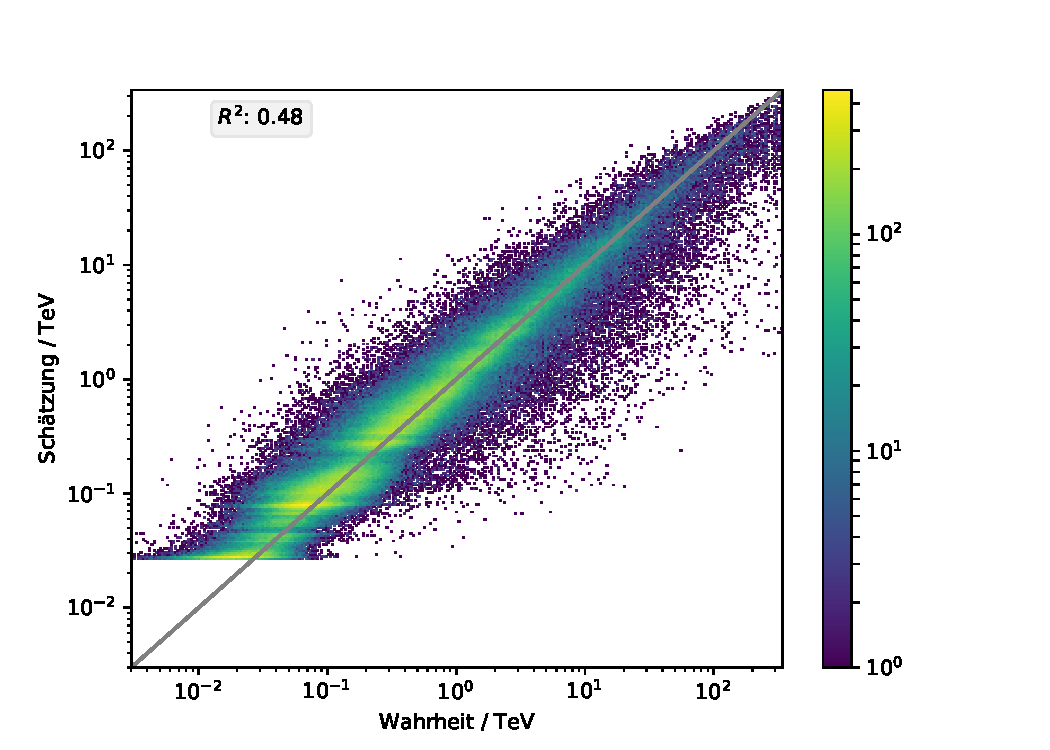
\includegraphics[width=1.1\textwidth]{pictures/trafo_encaps.pdf}
        \caption{Mit Transformation}
        \label{}
      \end{figure}
    \end{columns}
  \end{frame}

  \begin{frame}
    \begin{columns}
      \column{0.5\textwidth}
      \begin{figure}
        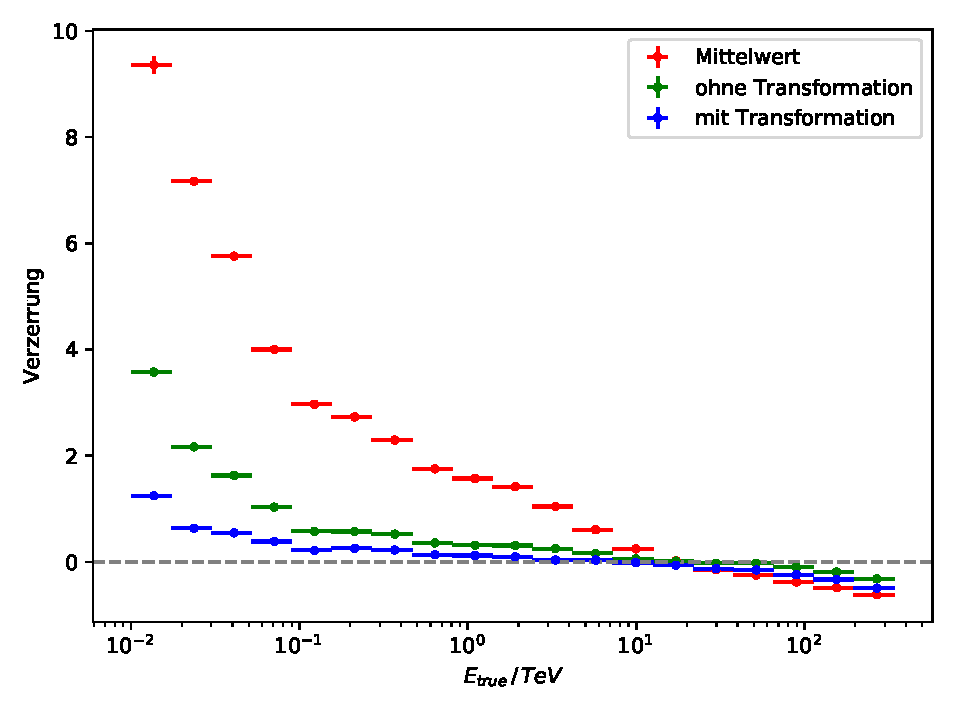
\includegraphics[width=\textwidth]{pictures/trafo_nested_bias.pdf}
        \caption{Mittelwert des relativen Fehlers für verschiedene Energiebereiche.}
        \label{}
      \end{figure}
      \column{0.5\textwidth}
      \begin{figure}
        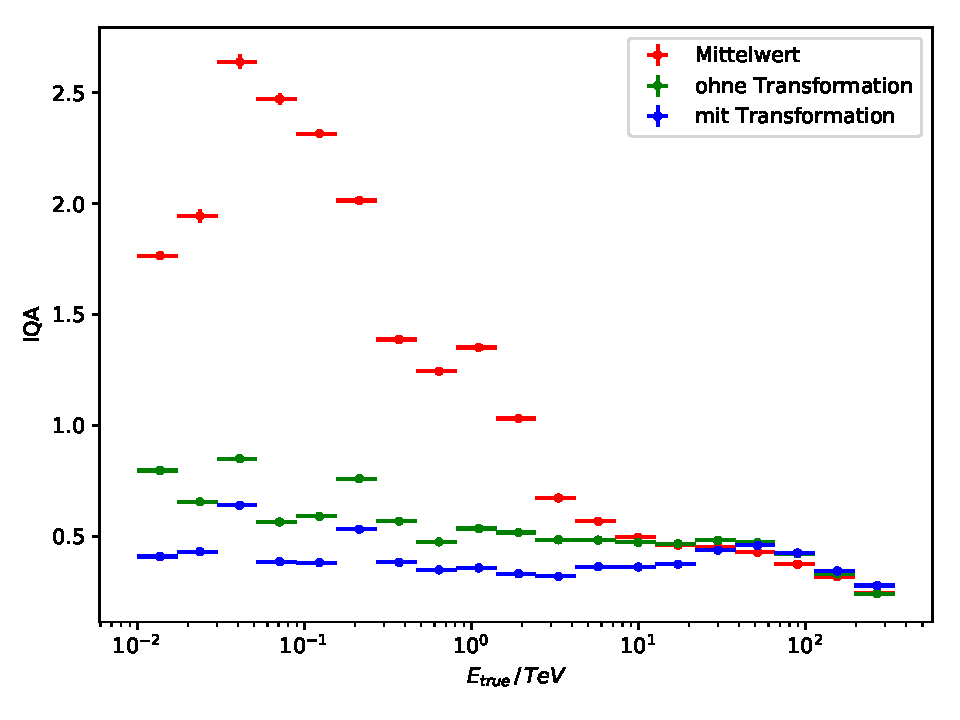
\includegraphics[width=\textwidth]{pictures/trafo_nested_resolution.pdf}
        \caption{Die Hälfte des IQA von $\SI{68,26}{\percent}$ des relativen Fehlers für verschiedene Energiebereiche.}
        \label{}
      \end{figure}
    \end{columns}
  \end{frame}

  \begin{frame}
    \frametitle{Absoluter Fehler}
    \centering
    Mittlere quadratische Fehler:
    \begin{equation*}
      \operatorname{mse} = \frac{1}{N} \sum_i (y_i-\hat{y}_i)^2
    \end{equation*}

    \vspace{0.9cm}

    \begin{tabular}{l|S}
      & $\operatorname{mse}$ \\
      \midrule
      Teleskopspezifische Schätzung & $\SI{102.94}{\tera\eV\squared}$ \\
      Arithmetisches Mittel & $\SI{65.31}{\tera\eV\squared}$ \\
      Median  & $\SI{66.61}{\tera\eV\squared}$ \\
      Gewichtung mit Intensität & $\SI{58.61}{\tera\eV\squared}$ \\
      Gewichtung mit Sensitivität & $\SI{64.72}{\tera\eV\squared}$ \\
      Eventspezifische Schätzung & $\SI{37.18}{\tera\eV\squared}$ \\
      \midrule
      \multicolumn{2}{l}{Transformation:} \\
      \midrule
      Teleskopspezifische Schätzung & $\SI{149.48}{\tera\eV\squared}$ \\
      Arithmetisches Mittel  & $\SI{94.60}{\tera\eV\squared}$ \\
      Eventspezifische Schätzung & $\SI{53.65}{\tera\eV\squared}$ \\
    \end{tabular}
  \end{frame}

  \section{Fazit}

  \subsection{Zusammenfassung}

  \begin{frame}
    \frametitle{Zusammenfassung der Ergebnisse}
    \begin{columns}
      \column{0.5\textwidth}
      \begin{itemize}
        \item Es wurden keine Cuts angewendet
        \item Anpassung der Methode auf die Aufgabenspezifische Analyse
        \item Beste Auflösung und geringste Verzerrung des relativen Fehlers bei der verschachtelten Methode mit Transformation
              Es könnte Verzerrung und Auflösung in weiten Bereichen um ca. $\SI{75}{\percent}$ gesenkt werden.
        \item Geringster mittlerer quadratischer Fehler bei der verschachtelten Methode ohne Transformation.
              Der absolute Fehler wurde um ca. $\SI{66}{\percent}$ gesenkt
      \end{itemize}
      \column{0.5\textwidth}
      \begin{figure}
        \centering
        \parbox{0.49\textwidth}{%
          \subfigure{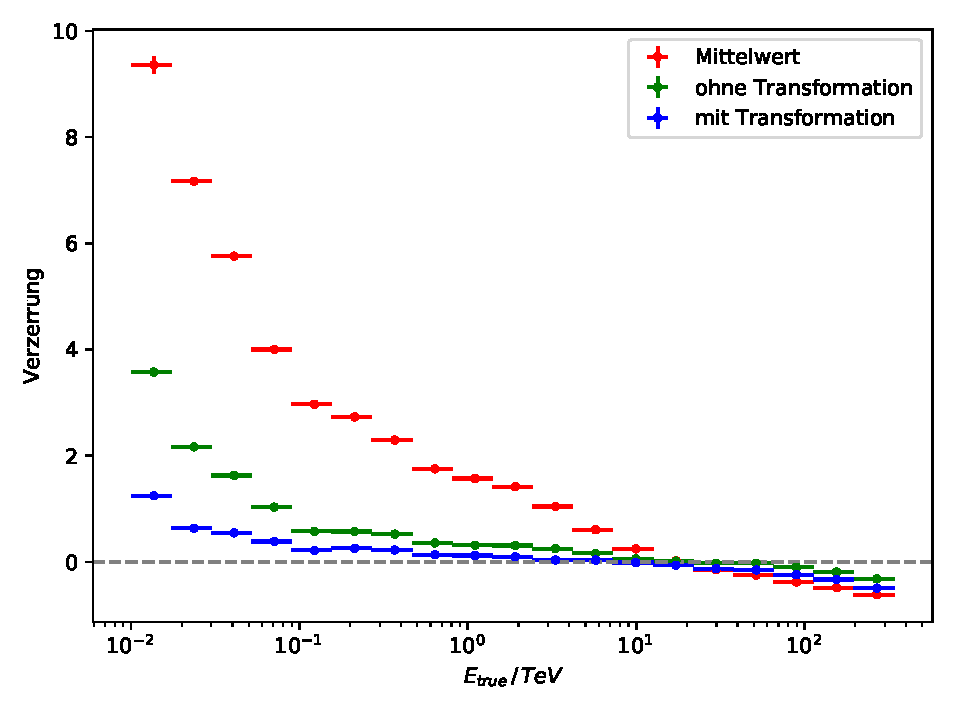
\includegraphics[width=0.55\textwidth]{pictures/trafo_nested_bias.pdf}}

          \subfigure{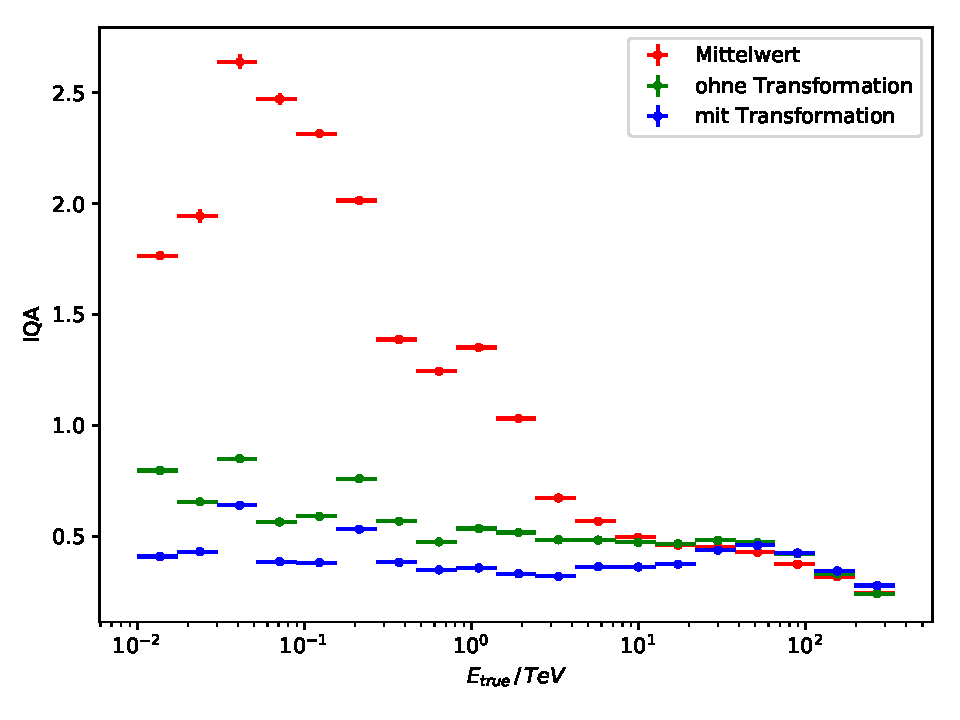
\includegraphics[width=0.55\textwidth]{pictures/trafo_nested_resolution.pdf}}}

      \end{figure}
    \end{columns}
    \begin{itemize}
      \item Es wurden keine Cuts angewendet
      \item Anpassung der Methode auf die Aufgabenspezifische Analyse
      \item Beste Auflösung und geringste Verzerrung des relativen Fehlers bei der verschachtelten Methode mit Transformation
            Es könnte Verzerrung und Auflösung in weiten Bereichen um ca. $\SI{75}{\percent}$ gesenkt werden.
      \item Geringster mittlerer quadratischer Fehler bei der verschachtelten Methode ohne Transformation.
            Der absolute Fehler wurde um ca. $\SI{66}{\percent}$ gesenkt
    \end{itemize}
  \end{frame}

  \subsection{Perspektiven}

  \begin{frame}
    \frametitle{Mögliche Perspektiven}
    \begin{columns}
      \column{0.5\textwidth}
      \begin{itemize}
        \item Abstand von Teleskop und Schauer und Höhe des Schauers als Attribut hinzunehmen
        \item Aufgabenspezifische Wahl der Transformation
        \item Kriterium für Entscheidungsbaum entwickeln welches den absoluten Fehler nutzt
      \end{itemize}
      \column{0.25\textwidth}
      \begin{figure}
        
\includegraphics[width=\textwidth]{pictures/sklearn.png}
      \end{figure}
      \begin{figure}
        
\includegraphics[width=\textwidth]{pictures/python.png}
      \end{figure}
      \begin{figure}
        
\includegraphics[width=\textwidth]{pictures/numpy.png}
      \end{figure}
      \column{0.25\textwidth}

      \vspace{0.6cm}

      \begin{figure}
        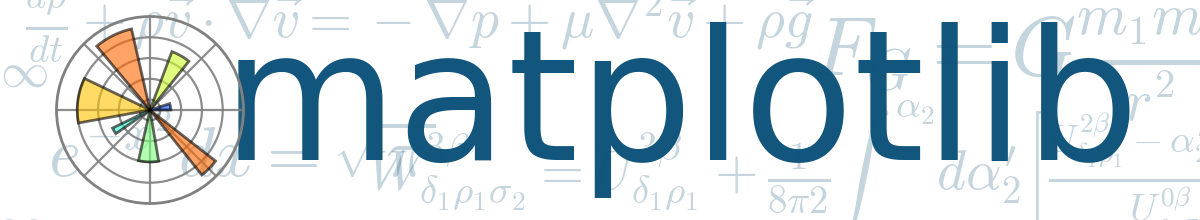
\includegraphics[width=\textwidth]{pictures/matplotlib.png}
      \end{figure}

      \vspace{0.6cm}

      \begin{figure}
        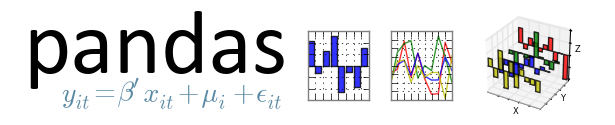
\includegraphics[width=\textwidth]{pictures/pandas.png}
      \end{figure}
    \end{columns}
  \end{frame}

  \section{}

  \begin{frame}[allowframebreaks]
    \printbibliography
  \end{frame}

  \begin{frame}
    \frametitle{Schauer Modell}
    \begin{figure}
      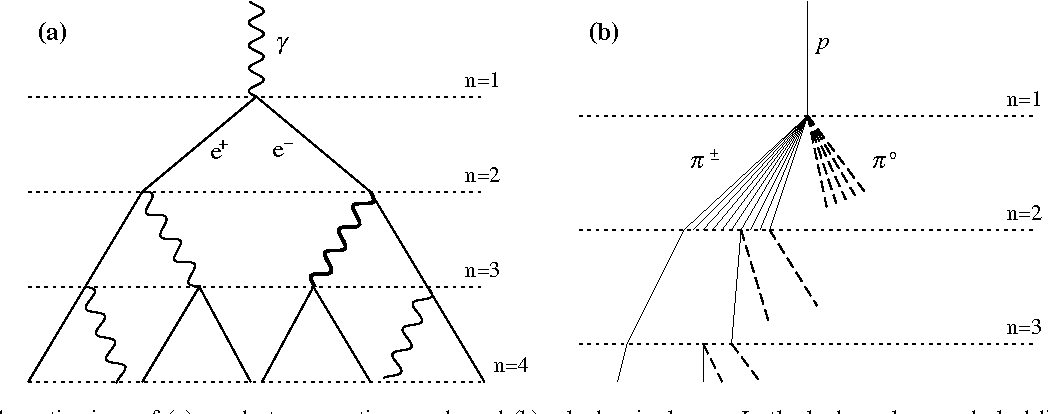
\includegraphics{pictures/Heitler.png}
      \caption{Joseph Matthews}
      \label{}
    \end{figure}
  \end{frame}

  \begin{frame}
    \frametitle{hallo}
  \end{frame}
\end{document}
